\documentclass[10pt,a4paper,twocolumn]{article}

\usepackage{graphicx}

\author {
  Thomas Haschka \and Joseph Bakarji
  }

\title{Semantic Tree Inference on Text Corpa using a Nested Density
  Approach together with Large Language Model Embeddings}

\begin{document}
\maketitle

\section*{Abstract}

Semantic text classification has undergone significant advances in
recent years due to the rise of large language models (LLMs) and their
high dimensional embeddings. While LLM-embeddings are frequently used to store
and retrieve text by semantic similarity in vector databases, the
global structure semantic relationships in text corpa often remains
opaque.

Herein we propose a nested density clustering
approach, to infer hirachical trees of semantically related texts. The
method starts by identifying texts of strong semantic similarity as it searches
for dense clusters in LLM embedding space. As the density
criterium is gradually relaxed, these dense
clusters merge into more diffuse clusters, until the whole dataset is
represented by a single cluster - the root of the tree. By embedding
dense clusters into increasingly diffuse ones, we construct a tree
structure that captures hierachical semantic relationships among texts.

We outline how this approach can be used to classify textual data for
abstracts of scientific abstracts as a case study. This enables the
data-driven discovery research areas and their subfields without
predefined categories. To evaluate the general applicability of the
method, we further apply it to established benchmark datasets such as
the 20 Newsgroups and IMDB 50k Movie Revies, demonstrating its
robustness across domains. 

Finally we discuss possible applications on scientometrics, topic
evolution, highlighting how nested density trees can reveal semantic
structure and evolution in textual datasets. 

\section{Background}

Text classification date back at least to bag of words models
\cite{bagofwords}. In these early approaches, each text is represented
as a vector of word frequencies, disregarding the order of words.
However, word order is a key semantic feature as changing it can
completely alter the meaning of a phrase. 

Subsequent refinements introduced term frequency and inverse document
frequency (tf-idf)
normalization \cite{tfidf}, which weights words by their relative
importance within a corpus. Later, Latent
Semantic Analysis (LSA) \cite{lsa-first,lsa,lsa-intro} applied
singlar value decomposition to capture latent relationships among
words and documents, enabling more robust document clustering and
topic modeling.
Easier to scale and based on probabilistic properties
instead of linear algebra Latent Dirichlet Allocation (LDA) \cite{lda}
and Hirachical Dirichlet Allocation (HDA) \cite{hda} have overtaken
the field of topic modelling. Neural network based approaches
such as word2vec \cite{word2vec} have arrived in the middle of the
last decade. These models could learn the relationships between words
in a semantic proximity sense, but still not in a grammatical
sequence.
The rise of the transformer model \cite{transformer} and the popularization
of LLMs allowed for the use of LLM embeddings for document
classification, and document retrieval. The transformer model is
superieur as it efficiently encodes and uses
the position of the words in the text as it generates embeddings. 
LLM embeddings have a such a vast field of applications and
\cite{llm-embed-chatbot,llm-embed-clust} commonly found in retrieval
augmented generation (RAG) pipelines \cite{rag,llm-embed-rag}.
All of the aforementioned methods project text into a mathematical
embedding space, where pairwise distances and clustering can be
applied to reveal latent semantic structures.
In parallel, hierarchical density clustering techniques have proven
highly effective in fields such as biological species classification,
phylogenetics \cite{mnhn-tree-tools}, and molecular dynamics, where
they are used to analyze protein conformations and structural
evolution \cite{md-tree-tools}.

Here, we extend these hierarchical density clustering methods to
textual embeddings, constructing tree-based representations of
semantically related texts. 
This approach goes beyond flat clustering by revealing how topics,
subjects, or emotions (depending on the embedding model) relate to one
another within a coherent hierarchical framework. 

\section{Introduction}

Topic modeling and semantic clustering have long aimed to uncover the
latent structure of large text corpora. With the rise of large
language models (LLMs) and their embeddings, it has become possible to
represent textual semantics with unprecedented precision. However,
most embedding-based clustering approaches produce flat partitions of
the semantic space, providing limited insight into how topics or
concepts are hierarchically related or evolve across scales.

In this work, we introduce a hierarchical density-based clustering
approach that infers tree structures from LLM embedding spaces. The
method builds upon previous applications of hierarchical density
clustering in bioinformatics and molecular dynamics, where it has been
successfully used to construct phylogenetic or conformational trees
from complex, high-dimensional data \cite{mnhn-tree-tools,
  md-tree-tools}. By adapting this framework to text embeddings, we
enable the reconstruction of semantic hierarchies. We show how dense
clusters of highly similar documents merge into broader, more diffuse
clusters as the similarity threshold is relaxed.

To construct such hierarchical structures, we employ a nested
density-based clustering procedure inspired by the DBSCAN algorithm
\cite{dbscan}. The core idea is to identify compact, high-density
regions of semantically similar embeddings and then progressively
relax the density criterion to reveal broader, more diffuse
groupings. This iterative relaxation enables clusters discovered at a
high-density level to merge into larger clusters at lower density
levels, naturally producing a hierarchical tree.
Formally, clusters of semantically similar texts that that
are densly connected in their respective embedding space are
determined by the condition:
\begin{equation}
  \rho_L > \frac{\mathrm{minpts}}{V(\epsilon_L)},
  \label{eqn-density-criterium}
\end{equation}
where $\rho_L$ represents the denstiy at a given iteration $L$. The
right hand side is given by starting parameters to the well known
Density-Based Spatial Clustering of Applications with Noise (DBSCAN)
algorithm \cite{dbscan}, with $\epsilon_L$ defining a radius at
iteration $L$ and $\mathrm{minpts}$ a minimum number of points within
this radius, effectively defining the density of a continious dense
ensemble to be found by the algorithm. To explore the semantic
structure at multiple scales, the radius $\epsilon_L$ is incrementally
expanded by a small step $\Delta\epsilon$ in each iteration. This
results in a sequence of density thresholds:  As $\epsilon$
increases, the volume in equation (\ref{eqn-density-criterium}) expands
leading to lower densities and
the identification of more diffuse clusters in each iteration. These
new clusters encapsulate denser ones from previous iterations,
allowing us to embed fine-grained semantic clusters into coarser ones,
thereby forming a hierarchical tree of semantic relationships. For a
subsequent layer (iteration) of the tree $L+1$ it follows, equation
(\ref{eqn-layers}):
\begin{equation}
  \rho_{L+1} > \frac{\mathrm{minpts}}{V(\epsilon_L+\Delta\epsilon)},
  \label{eqn-layers}
\end{equation}
or alternatively $\epsilon_L = \epsilon_{L-1} + \Delta \epsilon$. In
our previous work \cite{mnhn-tree-tools}, we demonstrated that using
this algorithm allows us to construct a hierarchical tree structure by
embedding dense clusters into progressively more diffuse clusters
until all elements of the conformational space merge into a single
cluster - the root of the tree. Figure
\ref{fig-tree-from-space} outlines the tree building procedure
conceptually. On the left, a text embedding space is shown, where each
colored sphere represents a piece of text. On the right the tree built
by the algorithm, from the text embedding space on the left, is shown. One can
observe how the graped, and orange colored texts fusion as the
density criteria is relaxed into the blue ensemble, encompassing both
clusters. At an intermediate step the green cluster stays separate,
while the rose texts are not encompassed and seen as outliers. Finally
as the density criterium is further relaxed all texts are only part of
one cluster, represented in gray on the right tree-outline. 
\begin{figure*}
  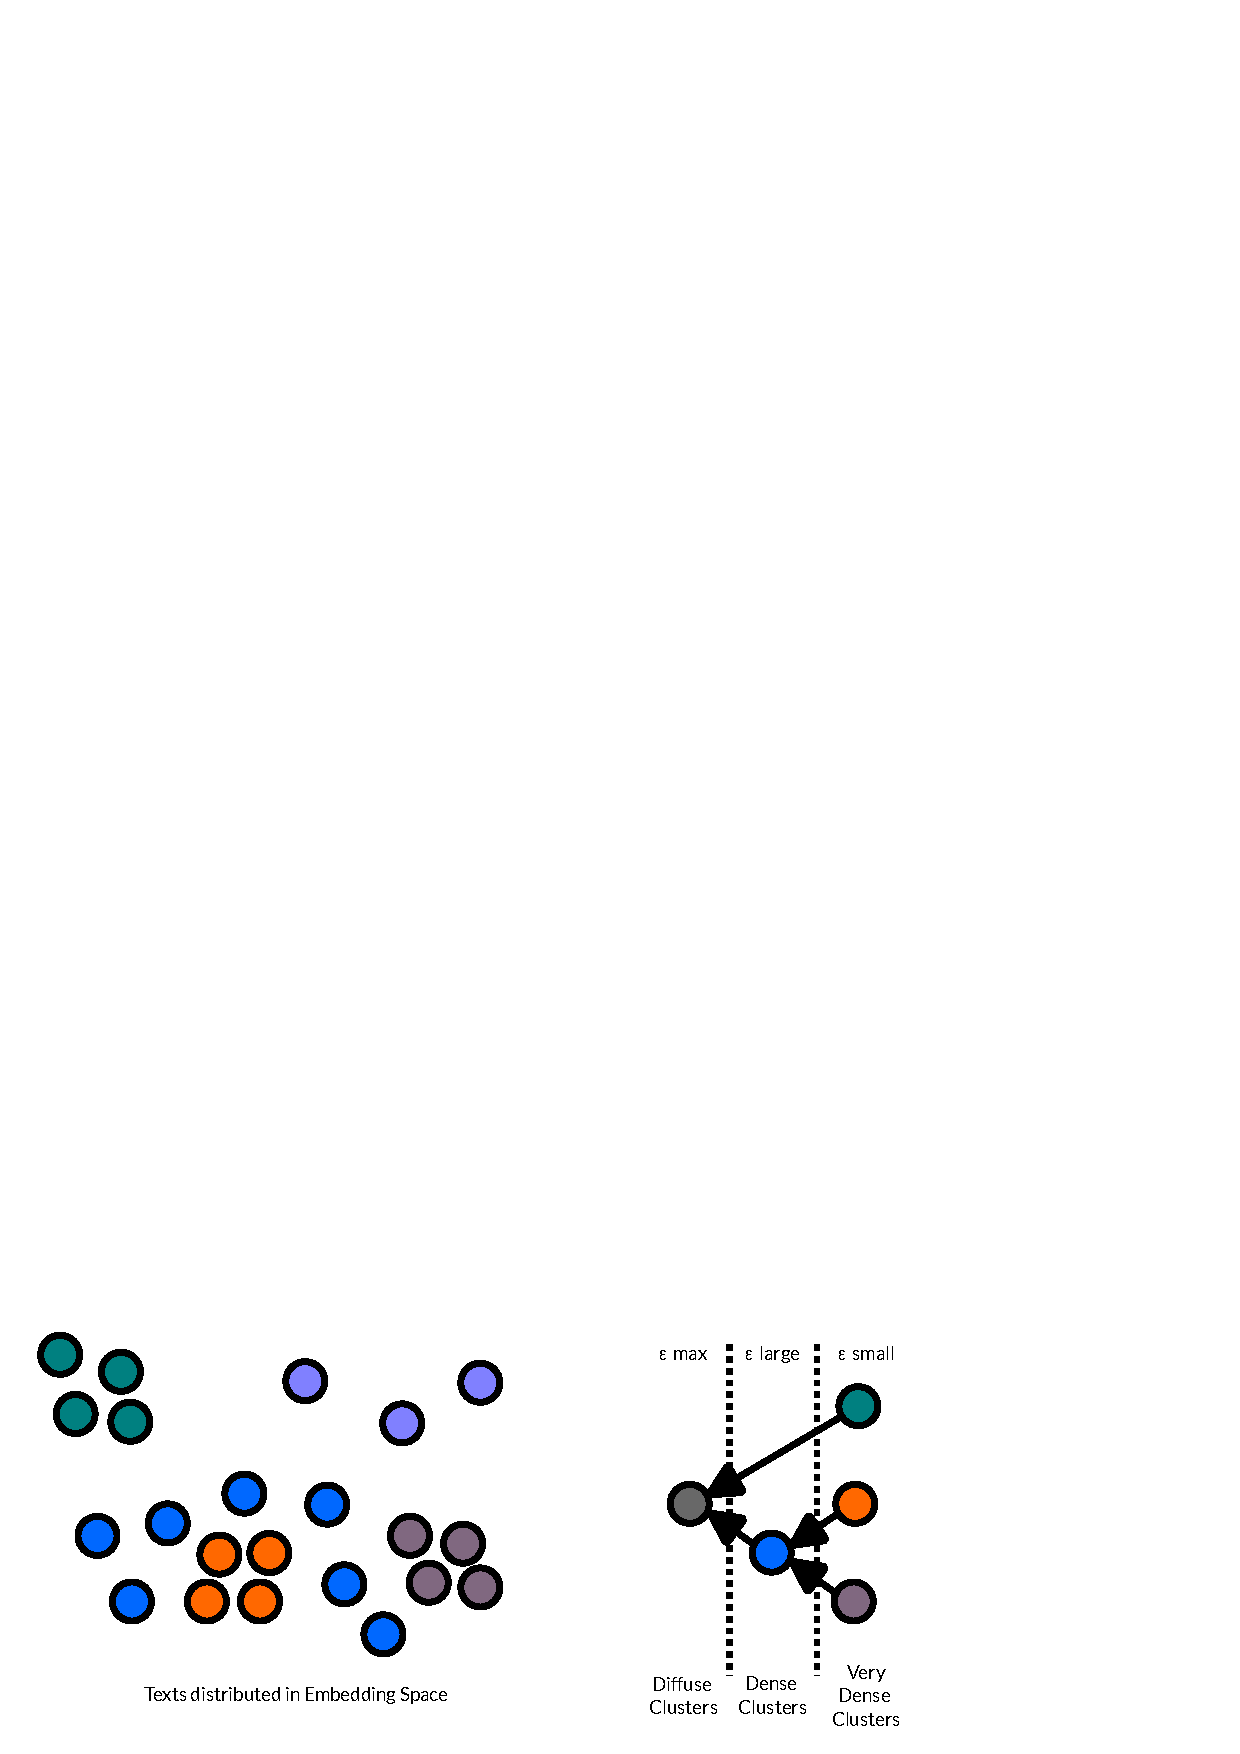
\includegraphics{tree-from-space.pdf}
  \caption{Tree building from a dataset reprented by its embedding
    space. On the left an embedding space with clusters of different
    densties is shown. One can see that the orange, and grape colored
    clusters embed into a larger blue ensemble. A conceptual tree
    built from such a two dimensional embedding space is shown on the right.}
  \label{fig-tree-from-space}
\end{figure*}
Our algorithm as such allows an organization for instance to show how
documents within the organization are related, finding clusters of
seperated by highly semantically similar documents, that merge, layer
by layer together to more diffuse clusters, until all documents form a
single cluster.

We demonstrate our approach on several corpora, including collections
of scientific abstracts and benchmark datasets such as 20 Newsgroups
and IMDB 50K reviews. In these experiments, we show how the inferred
semantic trees capture both fine-grained clusters of related documents
and higher-level thematic organization. Applied to the publication
records of institutions such as TU Wien and the American University of
Beirut, our method reveals naturally emerging research areas and
structural relationships between topics.

Once a semantic tree is constructed, an important challenge lies in
interpreting and annotating its clusters. We address this by
leveraging LLMs themselves: by prompting a model with the text content
of each cluster, we can automatically generate concise, human-readable
summaries or titles for each node in the hierarchy. This creates an
interpretable and fully automated pipeline for semantic structure
discovery in large text corpora.

\section{Materials and Methods}

\subsection{Datasets} \label{sec-datasets}

The primary goal of this study was to develop a pipeline for the
automated classification of research fields based on textual
similarity. While motivated by this scientific application, the
proposed approach is general and can be applied to a broad range of
text corpora. To ensure linguistic consistency and to avoid potential
errors caused by multilingual embeddings and the tree building
process, which would in such a case probably attributed different
branches to different languages, we restricted our analysis
to texts written in English.

We selected the following datasets for our study:
\begin{itemize}
  \item \textbf{Theses-fr-en}: English abstracts of theses defended in
    France: The French
    government publishes by means of its open data initiative a
    dataset containing all theses defended in France since 1985. We
    filtered this dataset for english abstracts. This data was
    obtained from the \emph{data.gouv.fr} platform.
  \item \textbf{TU Wien}:   English abstracts of publications affiliated
    with TU Wien between 2018 and April 2025. The data were provided by
    the TU Wien Service Unit for Research Information Systems as
    aggregated extracts from the institutional repository
    (\emph{reposiTUm}), Scopus, and Dimensions databases. Duplicates
    were removed, and only records containing English abstracts were
    retained. 
  \item \textbf{AUB}: English abstracts of publications authored by the
    American University of Beirut (AUB) from 2018 to October 2025. The data
    were provided by the AUB University Libraries. To ensure comparability,
    the roughly the same temporal window and language filters, only english
    abstracts, as for the TU Wien corpus were applied.
  \item \textbf{20 Newsgroups}: The 20 Newsgroups dataset is a widely
    used benchmark corpus for 
    text classification and topic modeling. It consists of
    approximately 20,000 newsgroup posts collected from 20 distinct
    discussion groups on topics such as science, politics, sports,
    religion, and technology \cite{20newsgroups}.
  \item \textbf{IMDB 50K Reviews}:
     A corpus of 50,000 movie reviews from
     the Internet Movie Database (IMDB), each labeled with a binary
     sentiment (positive or negative) \cite{50kmovies}. 
   \item \textbf{AG News}: A large-scale news dataset consisting of short
     article titles and descriptions categorized into four topics: World,
     Sports, Business, and Science/Technology.
     \cite{agnews}. 
  \item \textbf{dbpedia\_14}: This dataset contains short texts
    labeled by 14 classes such as: as Company, Educational
    Institution, Artist, Athlete, Office Holder, and Place
    \cite{agnews}. It serves as a large-scale evaluation corpus for
    general semantic representation.
\end{itemize}
Statistics about the different datasets are shown in table
\ref{tab-dataset-statistics}.

\begin{table}
  \begin{center}
  \begin{tabular}{l|rrr}
    & n(Texts) & mean & stddev \\
    \hline
    theses-fr-en & 180939 & 261.89 & 112.70 \\
    TU Wien & 27506 & 168.85 & 73.79 \\
    AUB & 15982 & 237.73 & 98.24 \\
    20newsgroups & 11314 & 287.47 & 541.46 \\
    50k-movies & 50000 & 231.16 & 171.34 \\
    ag\_news & 127000 & 37.84 & 10.09 \\
    dbpedia\_14 & 630000 & 46.13 & 22.46 
  \end{tabular}
  \caption{Statistics about the text corpa used. \emph{n(Texts)} is
    the number of unique texts in the dataset, \emph{mean} and
    \emph{stddev} represents the mean and standard deviation of the
    number of words contained in each text of the dataset.}
  \label{tab-dataset-statistics}
  \end{center}
\end{table}
    
\subsection{Embeddings}
Embeddings for the datasets outlined in section \ref{sec-datasets}
were generated using either the Qwen3-Embedding-8B
\cite{qwen3embedding} or SFR-Embedding-Mistral \cite{SFRembedding}
model. These models were chosen selected based on their high performance in the
MTEB-Leaderboard found on Huggingface, and the their practical
deployability on the computing infrastructure accessible to us.

4096 dimensonal embedding vectors obtained for each text from a
dataset were stored in an in house developed vector database.

Each text sample was transformed into a 4096-dimensional embedding
vector. The resulting embeddings were stored in an in-house developed
vector database optimized for high-throughput semantic similarity
retrieval.

\subsection{Tree Building}

\subsubsection{Pairwise Distance and Dimensionality Reduction}

The pairwise distance between embeddings serves as the foundation for
the hierarchical tree construction process. We employed the cosine
distance on the full-length embedding vectors as well as the $L_2$-norm
on reduced-dimensional representations obtained via Principal
Component Analysis (PCA). 

Dimensionality reduction proved crucial, as PCA functions as a feature
selection mechanism that prioritizes components with maximum variance.
Empirically, we observed that reducing the number of components leads
to more clearly separated and interpretable cluster structures. While
the original embedding vectors contain 4096 dimensions, spectral
analysis indicated significant redundancy among components. The choice
of the number of principal components thus directly affects the
resolution and spread of the resulting semantic tree.

\subsubsection{Adaptive Density Clustering with DBSCAN}

For each dataset, we constructed trees using an adaptive density-based
clustering procedure built upon successive runs of the DBSCAN
algorithm. Each DBSCAN iteration identifies clusters at a specific
density level, controlled by a triplet of parameters: the initial
neighborhood radius $\epsilon_0$, the incremental radius step
$\Delta\epsilon$, and the minimum number of points within the radius
($\mathrm{minpts}$). 

In each successive run, the radius is increased by $\Delta\epsilon$
while keeping $\mathrm{minpts}$ constant. This progressively lowers
the effective density threshold and allows previously dense clusters
to merge into more diffuse ones. Whenever the number of clusters found
in a given iteration is smaller than in the preceding step, the newly
identified clusters are stored, and the clusters from the prior
iteration are embedded within them. This iterative embedding process
builds the hierarchical tree structure described in
Figure \ref{fig-tree-from-space}, where dense clusters at outer layers
merge stepwise into broader, semantically diffuse clusters toward the
root.

\subsection{Tree Annotation}

The resulting trees consist of multiple hierarchical layers. Each
layer represents a set of clusters that form the nodes at that level,
while edges connect clusters of higher density (outer layers) to
broader, lower-density clusters (inner layers). This structure allows
fine-grained semantic groups to merge progressively into coarser
domains.

To realize our goal of a data-driven research field classification
pipeline, we sought to automatically annotate each node with a
representative topic label. The underlying assumption is that smaller,
high-density clusters correspond to specialized research areas, while
broader clusters capture more general scientific domains.

To generate these annotations, we employed a Large Language Model
(LLM) capable of handling large textual contexts. Specifically, we
used the Llama-4-Scout-17B-16E-Instruct model
\cite{meta2024llama4} in 6-bit quantized form,
which provides a nominal context window of up to
11 million tokens. Due to technical constraints, our inference
pipeline successfully operated with a maximum context size of
approximately 600,000 tokens.

Both the TU Wien and AUB corpora were fully annotated, encompassing
all English-language scientific abstracts published since 2018. For
each node, the LLM received the text of all abstracts within that
cluster and was prompted to infer a unifying research field label. 

In cases where a cluster contained more than 1500 abstracts (exceeding
the 600,000-token limit), we randomly sampled 1500 abstracts per
processing chunk. For $n$ total abstracts in a cluster, the number of
chunks $s$ was determined as:
\begin{equation}
  s = \frac{3n}{1500},
  \label{eqn-sampling}
\end{equation}
where the factor of 3 ensures oversampling to enhance topic stability.
Each chunk was processed independently by the LLM to yield a candidate
research field label. In less then 1 in 100 cases, the LLM did not
produce a clear output. Even though the prompt enforces to yield only
one research field on a single line, this is not always the case. As
such in all cases where answers span more than one line, or contain
more than 80 characters, we
yield these answers to the gpt-oss-20b model \cite{gpt-oss} in 8-bit
quantized form, and ask it
to decide from the previous output on a single research field. As the
output from the first run might be due to errors in the LLM very large
we only keep the last 20000 characters during this pass to the
gpt-oss-20b model. 

In the case were the cluster had to be sampled because it contained
more than 1500 abstracts all resulting labels were subsequently fed into
a second LLM pass. Again the gpt-oss-20b model \cite{gpt-oss} in 8-bit
quantized form is used in such a case where the model inferred the
overarching research field encompassing all $s$ subfields. An overview about
the different paths that annotation might undergo is outlined in Figure
\ref{fig-annotation}.
\begin{figure}
  \begin{center}
    
\includegraphics{annotation-schema.pdf}
    \caption{Shematic represantation of the tree node / cluster
      annotation process}
    \label{fig-annotation}
  \end{center}
\end{figure}
  

Tree annotation is computationally intensive. The AUB tree required
annotating 33{,}862 text files, while the TU Wien tree required
62{,}012, including oversampling according to
Equation~\ref{eqn-sampling}. Inference was performed using the
\texttt{llama.cpp} \cite{llama-cpp} engine on the MUSICA supercomputer
(Austria). Up to 80 NVIDIA H100 GPUs were employed concurrently during
annotation. Each compute node with four H100 GPUs (80~GB VRAM each)
handled batches of approximately 600{,}000 tokens per inference
instance. Multi-node inference, which could allow for a higher context
token limit, was not attempted as MUSICA is currently in its test
phase; instead, parallelism was achieved by distributing text files
across multiple nodes for simultaneous inference.

\subsection{Label Transcription}

The theses-fr-en dataset is annotated and contains a research field
(discipline, in French) for each abstract. However, these fields can
in many cases be freely chosen by the thesis author, resulting in 13,599
unique discipline labels. 
To obtain a more coherent and standardized annotation, we used the
gpt-oss-20b model to classify all 13,599 labels according to the
OECD Fields of Science (FOS) 2002 classification \cite{oecd-fos}. 
The resulting transcribed labels were then used to color
the trees inferred from this dataset, allowing us to assess whether
specific scientific fields tend to separate into distinct
and meaningful branches. 

\subsection{Tree Coloration and Visualization}

To facilitate interpretation and qualitative validation of the inferred
trees, we applied coloration schemes that project existing labels or
metadata onto the tree structure. This process enables us to visualize
how known categories or attributes distribute across different branches
of the tree.

For example, in the case of the 20~Newsgroups dataset, tree
coloration reveals how posts from individual newsgroups are positioned
within the hierarchical semantic structure. Similarly, for the
TU~Wien dataset, coloration based on existing research
classifications allowed us to assess how well our hierarchical density
clustering recovers semantically coherent domains.

Tree coloration was performed using utilities provided by
MNHN-Tree-Tools \cite{mnhn-tree-tools}. In particular, we
employed the \texttt{tree\_map\_for\_split\_set} tool to map predefined
clusters or labeled subsets onto the corresponding nodes of the
hierarchical tree. The resulting color maps were generated for
visualization using the newick-utilities package
\cite{newick-utilities}, a software suite for the manipulation and
visualization of phylogenetic trees.

This approach allowed us to produce colored tree visualizations for
each dataset. In the 20 Newsgroups case, individual trees were
colored according to each newsgroup category, highlighting topic
segregation and overlap. For the IMDB 50K reviews dataset, we colored
the tree by sentiment polarity, enabling a visual inspection of how
positive and negative reviews cluster across different density layers.

\section{Results}

\subsection{Efficiency of PCA and the $L_2$-norm Compared to Cosine Distance}

Cosine distance is widely used for comparing high-dimensional embedding
vectors and is the default similarity measure in many retrieval-based
applications, including RAG pipelines. For this reason, we initially
expected cosine distance to be the natural choice for the DBSCAN
iterations underlying our tree construction algorithm. However, trees
constructed directly from full 4096-dimensional cosine distances
consistently exhibited limited structural resolution: branches were
poorly separated, fine-grained clusters failed to emerge, and the overall
tree topology did not yield significant insights.

In contrast, applying Principal Component Analysis (PCA) prior to
clustering dramatically improved the quality and expressiveness of the
resulting trees. Experiments with 10, 5, and 2 principal components
showed that lower-dimensional PCA representations consistently produced
more “spread out” trees with clearer branching and more detectable
fine-scale semantic substructure. We suggest that this effect is due
to the inherent ability of PCA to yield principal components that
maximize variance and that this feature selection process has a
positive effect on our clustering algorithm. A similar effect was
noted previously in the algorithmic supplement of
\cite{mnhn-tree-tools}.

A comparison between trees obtained with cosine distance and with the
$L_2$-norm applied to PCA-reduced embeddings is shown in Figure
\ref{fig-compairison-L2-cos}. From left to right, the trees become more
hierarchically detailed and reveal progressively finer semantic
subclusters. For these illustrative examples, the parameters were chosen
using a rudimentary bisection search to produce visually optimized
trees. The parameter settings were as follows: for cosine distance,
initial $\epsilon = 0.275$, $\Delta \epsilon = 0.001$, and
$\mathrm{minpts}=5$; for the $L_2$-norm on 10 principal components,
initial $\epsilon = 0.091$, $\Delta \epsilon = 0.0001$,
$\mathrm{minpts}=5$; and for the $L_2$-norm on 2 principal components,
initial $\epsilon = 0.0039$, $\Delta \epsilon = 0.00001$,
$\mathrm{minpts}=5$. The trees shown in \ref{fig-compairison-L2-cos}
were built from embeddings obtained form the Qwen3-Embedding-8B model.
\begin{figure*}
  \begin{center}
  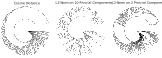
\includegraphics{comparision-cos-L2.pdf}
  \caption{A comparison of trees built from the 20 Newsgroups dataset
    under different distance measures}
  \label{fig-compairison-L2-cos}
  \end{center}
\end{figure*}

\subsection{Detection of Topics and Semantics}

Depending on the dataset, we applied different evaluation strategies to
assess whether, and to what extent, the method proposed in this work
produces meaningful and reliable results, given the computational
constraints of our setup. The following subsections outline these
evaluations and illustrate the behavior of our hierarchical
density-based tree construction across diverse text corpora.

\subsubsection{20 Newsgroups}

To evaluate whether our tree construction method recovers meaningful
semantic structure, we applied it to the 20 Newsgroups dataset. The
resulting trees were colored according to posting labels, as shown in
Figure \ref{fig-20news-colored}. For each newsgroup we generated a
separate color map: posts from the target newsgroup are shown in blue,
and posts from all other newsgroups in orange. Both color intensities
follow a logarithmic scale proportional to the number of posts in each
cluster, with white indicating the absence of posts of a given type.

The inferred tree, as highlighted in figure \ref{fig-20news-colored},
recovers many interesting relationships between the newsgroups:

\begin{itemize}
\item \textbf{Sports-related groups.}  
  The groups \emph{rec.sport.baseball} and \emph{rec.sport.hockey}
  form a shared subtree located close to the root of the full tree.
  This indicates strong internal similarity between the two sports
  discussions, combined with substantial separation from most other
  topics.

\item \textbf{Automotive-related groups.}  
  The groups \emph{rec.autos} and \emph{rec.motorcycles} cluster
  tightly in a small dedicated sub-branch. A fraction of their posts
  appears in regions of the tree that correspond to scientific or
  technical discussions, likely reflecting threads involving
  engineering aspects of vehicles.

\item \textbf{Religion and politics.}  
  The groups \emph{soc.religion.christian}, \emph{alt.atheism}, and
  \emph{talk.religion.misc} form a joint subtree that also contains
  the political groups \emph{talk.politics.guns},
  \emph{talk.politics.mideast}, and \emph{talk.politics.misc}.  This
  intersection reflects the topical proximity and overlapping
  discussions between religion and politics within the dataset.

\item \textbf{Computer-related groups.}  
  The \emph{comp.*} groups, including \emph{comp.sys.mac.hardware},
  \emph{comp.windows.x}, \emph{comp.graphics}, and
  \emph{comp.os.ms-windows}, form a coherent subtree corresponding to
  computer hardware and software discussions. Some overlap with
  \emph{sci.electronics} is visible, consistent with semantically
  similar content.

\item \textbf{Marketplace group.}
  The \emph{misc.forsale} posts distribute across multiple regions of
  the tree, often co-occurring with the automotive and computer
  subtrees, suggesting that sale-related messages tend to mirror the
  underlying topical focus of corresponding technical groups.

\item \textbf{The cryptography group.}  
  The \emph{sci.crypt} group appears in a distinct set of branches
  close to the root, and is clearly separated from both the scientific
  and computer-related subtrees. This separation may stem from the
  unique vocabulary and specialized discourse typical of cryptography
  discussions.
\end{itemize}

Overall the structure seems to intuitively make sense, outlining
intervoven fields of discussion. Importantly,
our toolchain does not merely cluster newsgroups into isolated groups;
it also conveys the relative proximity and semantic distance between
them. The resulting tree therefore serves as a compact visual
instrument that captures both fine-grained cluster structure and the
broader topology of topic similarity within the dataset, all within a
single interpretable representation. 
\begin{figure*}
  \begin{center}
    \includegraphics{20-newsgroups.pdf}
    \caption{Tree represenations of the 20 Newsgroups dataset.}
    \label{fig-20news-colored}
  \end{center}
\end{figure*}

\subsubsection{IMDB 50K Reviews}

The IMDB 50K Reviews dataset was used to evaluate whether our tree
construction method, together with the underlying embedding models, is
able to separate reviews by emotional polarity. We therefore built a
tree from this dataset following the same procedure as for the other
corpora. The resulting tree was then colored analogously to the 20
Newsgroups experiments: clusters containing predominantly positive
reviews were assigned a blue shading, while clusters containing
predominantly negative reviews were shaded in orange. As before, color
intensity follows a logarithmic scale, with white indicating the
absence of reviews of a given label and deeper blue or orange
indicating higher concentration. Overlaps appear in darker,
greenish to black tones. 

The resulting tree is shown in Figure
\ref{fig-50k-news-colored}. Compared to the other datasets, the IMDB
tree appears noticeably less structured, suggesting that the
underlying corpus is more homogeneous and lacks strong semantic
subdivisions beyond sentiment. Nonetheless, we observe a few small
subtrees near the periphery of the tree in which positive reviews form
a clear majority. Additional localized regions with a majority of
positive or negative reviews can also be identified. We speculate that
these structures arise from repetitive linguistic patterns that occur
more frequently in either positive or negative reviews. However, they
do not form large coherent branches, and overall the dataset does not
separate cleanly by sentiment. 

This observation suggests that the embedding models
used: Qwen3-Embedding-8B \cite{qwen3embedding} and
SFR-Embedding-Mistral \cite{SFRembedding} encode emotional polarity
only to a limited extent. The results highlight the importance of
choosing embedding models appropriate for the expected semantic
structure when constructing trees. 

We also attempted to annotate the IMDB tree with the
Llama-4-Scout-17B-16E-Instruct model \cite{meta2024llama4}. The goal
was to obtain genre-level descriptions of tree regions, under the
assumption that certain movie genres might correlate with
predominantly positive or negative reviews. This attempt was
unsuccessful: the model did not produce reliable or meaningful genre
assignments, and more fundamentally, such information appears to be
largely absent from the review text itself. As such, deriving movie
genres from this dataset seems infeasible with current methods. 
\begin{figure}
  \begin{center}
    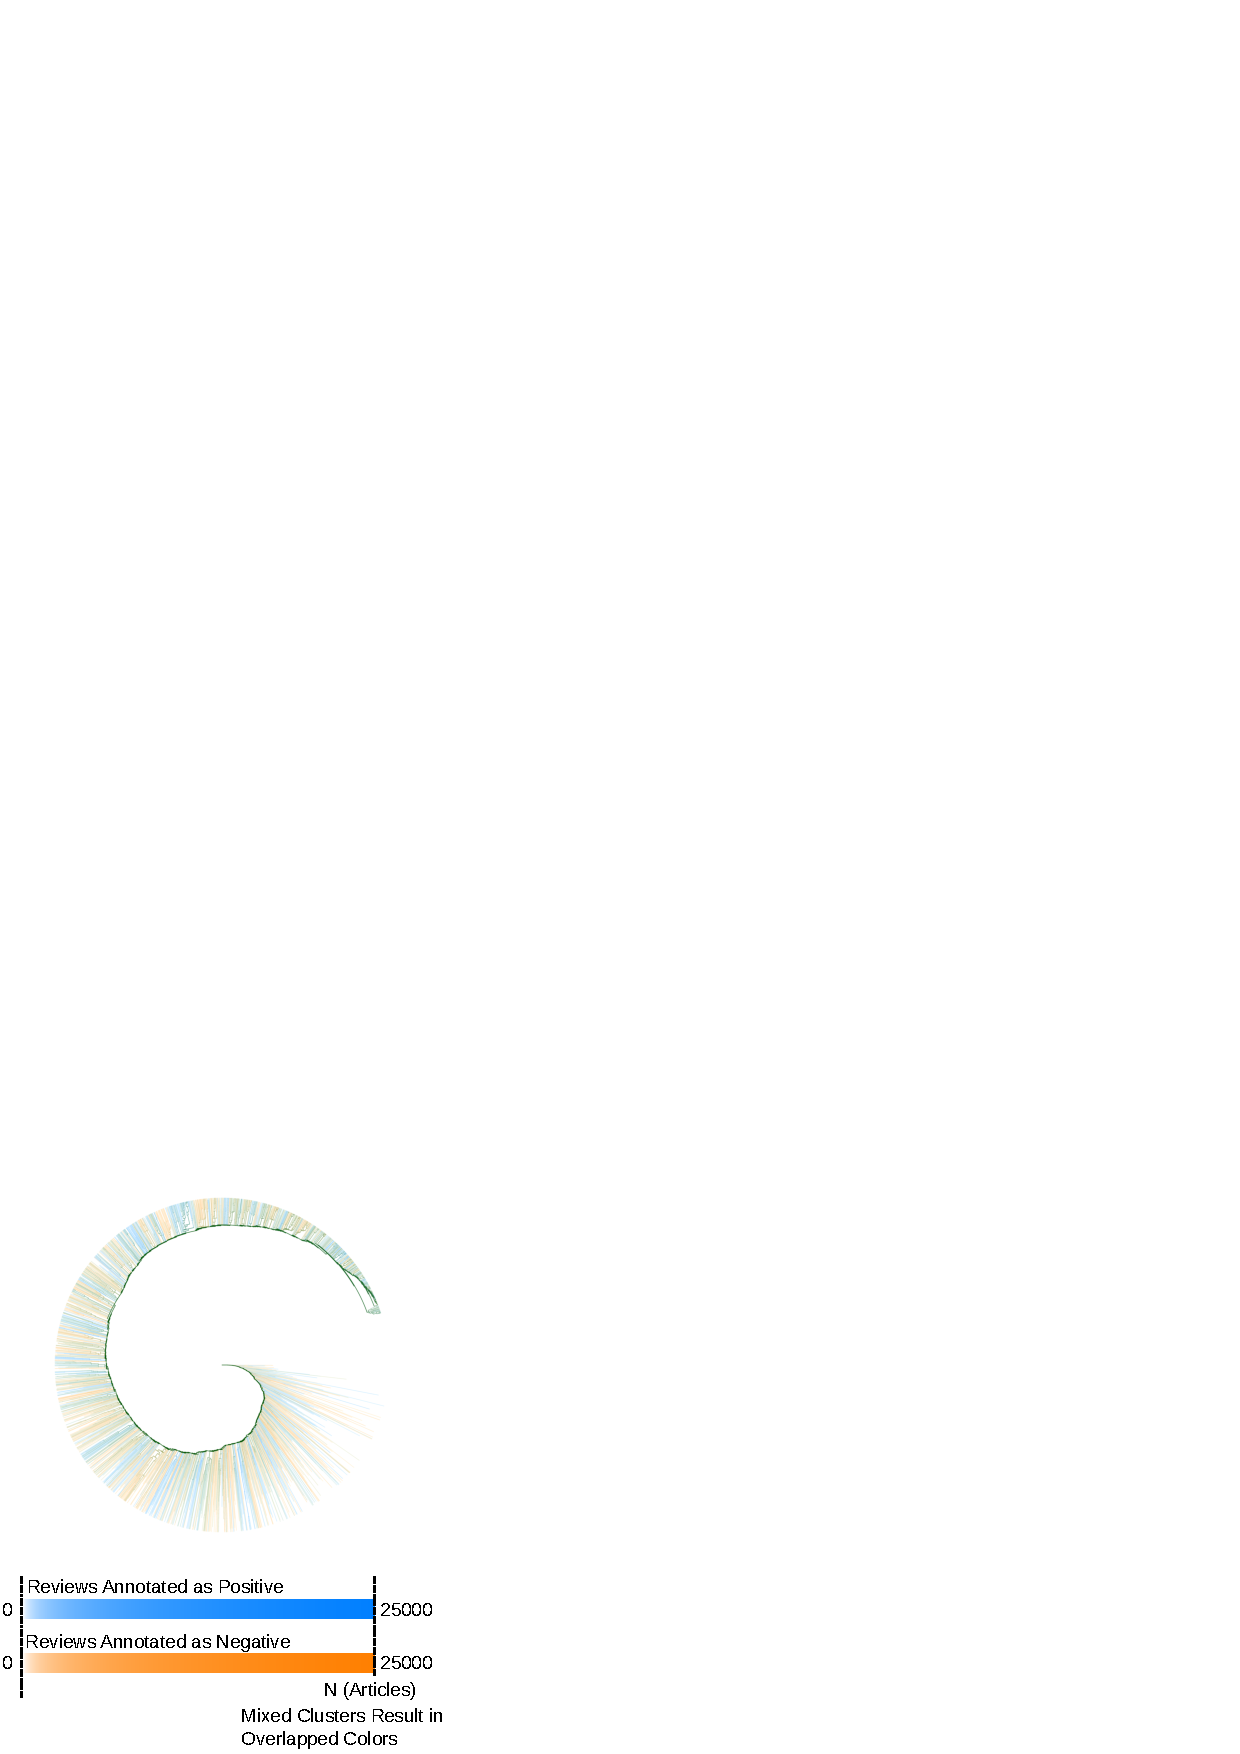
\includegraphics{50-pos-neg.png}
    \caption{The IMDB 50K Reviews dataset colored by sentiments.}
    \label{fig-50k-news-colored}
  \end{center}
\end{figure}

\subsubsection{AG News}

We further built trees from the AG News dataset and colored them
according to the four available labels: World, Sports, Business, and
Science/Technology. For each label, a separate color map was generated.
Items belonging to the target label are highlighted in blue, while all
other items are shown in orange. As in previous visualizations, we use a
logarithmic color gradient to represent the number of articles in each
cluster, ranging from white (no articles of that type) to fully saturated
colors (all articles in the cluster belong to the target label). The
resulting trees are shown in Figure \ref{fig-ag-news}. 
\begin{figure*}
  \begin{center}
    \includegraphics{ag_news.pdf}
    \caption{Trees built from the AG News dataset.}
    \label{fig-ag-news}
  \end{center}
\end{figure*}
We observe that the world and sports categories form
clearly separable structures: both branch off early from the root of the
tree, resulting in two well-defined clades with only minimal
contamination from other labels. Around the root, however, a small number
of scattered articles appear, suggesting that certain headlines are not
easily classifiable by the embedding models. These headlines seem to be
very distant from the other news items, only joining the root at a
very diffuse density.

The remaining two categories, business and science/technology, show
substantial overlap. They jointly occupy the third major branch of the
tree, and only small terminal sub-branches demonstrate consistent
label-specific structure. We attribute this to the general type of
embedding models that we are using here and that business headlines
frequently mention science and technology and vice versa in this
dataset. 

\bibliographystyle{ieeetr}
\bibliography{bib}

\end{document}
